\documentclass[11pt]{article}
\usepackage[scaled]{helvet}
\renewcommand\familydefault{\sfdefault} 
\usepackage[T1]{fontenc}%%% use with PDFLaTeX
\usepackage[utf8]{inputenc}
\usepackage[top=25mm,left=25mm,right=25mm,bottom=20mm,headsep=15pt,footskip=15pt,a4paper]{geometry} % see geometry.pdf on how to lay out the page. There's lots.
\usepackage[english]{babel}
\usepackage{color}
\usepackage{enumitem}
\usepackage[colorlinks,citecolor=blue]{hyperref}
\usepackage[parfill]{parskip} % no indentation
\newcommand\todo[1]{\textcolor{red}{#1}}
\usepackage[backend=biber,style=authoryear, dashed=false]{biblatex}
\emergencystretch=1em
\usepackage{graphicx}
\usepackage{amsmath}
\usepackage{amssymb}
\usepackage{subfig}
\usepackage{booktabs, dcolumn, caption, bm}
\usepackage{makecell}
\newcolumntype{d}[1]{D{.}{.}{#1}} % "decimal" column type
\renewcommand{\ast}{{}^{\textstyle *}} % for raised "asterisks"
\graphicspath{ {./figures/} }
\usepackage{wrapfig}
\usepackage{booktabs}
\addbibresource{references.bib}


\makeatletter         
\def\@maketitle{   % custom maketitle 
\begin{center}%
{\bfseries \@title}%
{\bfseries \@author}%
\end{center}%
\smallskip \hrule \bigskip }


\title{{\LARGE Coreference Resolution}\\[1.5mm]
{\large Working Title, First Draft: Content, not Wording}\\[1.5mm]} %%% Span Representation And Long-Range Coreference
%% Exploring Span Representations in Neural Coreference Resolution?
\author{Patrick Kahardipraja, Olena Vyshnevska}%%% Fill in your name 
\date{} % delete this line to display the current date


%%% BEGIN DOCUMENT
\begin{document}

\maketitle


\section{Introduction}

% Main contribution: Dissect Span representation using probing model, show what is useful, in particular w.r.t the effect of fine-tuning 

% Role of Coreference Resolution in NLP . 
%Some nice long paragraphs about place of coreference in NLP  
Coreference Resolution (CR) is a vital part of Natural Language Understanding and Natural Language Processing (NLP). It's applications include information extraction, question answering, summarization, machine translation, dialog systems etc. The task consists of mention detection and mention clustering. Some systems only focus on one part, while others propose end-to-end solutions.

The notion of mention -- a span of text referring to some entity -- is central to the task of CR. Mentions can be one of the three kinds: pronouns, named entity, and noun phrases. When several mentions \textit{corefer} they refer to the same entity. 

Since the seventies automated solutions for coreference resolutions have been researched \parencite{woods1972, winograd1972, hobbs1978}. Some of the challenges central to the field include semantic and syntactic agreement between mentions; encoding non-local dependencies; paraphrasing of repetitions.


% While being a language short of elaborate agreements, English certainly enjoys the most scientific attention. It is a known challenge in NLP to do more research with agreement-rich languages \textit{citation needed}. 

% Challenges in the Field . 
% Paragraphs about problems with coref   
% Narrow down to loca/non-local coreference . 

% Our Proposed Solution
% Very broadly what we intended to to

Since the introduction of pre-trained BERT model  \parencite{devlin2019bert} there has been a lot of research showing how the model outperforms previous state-of-the-art task-specific NLP models. \todo{cite some papers here} % cite more papers here 
\textcite{joshi2019coref} has introduced BERT models into coreference resolution tasks. However, the researchers have also encoded other information on top of BERT embeddings. 

Our first research question is based on the recent research which shows that the BERT model itself encodes a significant amount of semantic and syntactic information. Therefore, we decided to test how well the span representations using BERT embeddings from the model by \textcite{joshi2019coref} finetuned on Ontonotes dataset \parencite{conll}  can encode coreference resolution information without any layers of additional information about a given sequence. 

As a baseline, we used original pre-trained BERT embeddings. To encode a mention span,  we used a convolutional layer and a  self-attention layer.

Our second research question, which naturally follows from the first one, whether the span representations encoded with a pre-trained BERT model simply modelling local coreference? Will it be able to encode non-local coreference dependencies? 

We found that the span represenations from within the coreference model by \textcite{joshi2019coref} reach \textit{insert some numbers}. The baseline model is at \textit{insert numbers}. This findings suggests that the pre-trained BERT model is a powerful tool for encoding information relevant to coreference resolution. 

For our second research question (non-local VS local dependencies) we found that ... \todo{what we found for local non-locat}

Our code is publicly available on GitHub.  \footnote{\url{https://github.com/alyonavyshnevska/bert_for_coreference_resolution}}.


\section{Related Work}

\subsection{Approaches to Coreference Resolution}
% Explain several types of approaches for coreference resolution with each difference, later link that we choose span-ranking models.
% find something about span representation?

%Architectures for coreference resolution models are typically categorized as 1) mention-pair classifiers \parencite{ng2002identifying, bengtson2008understanding}, 2) mention-ranking classifiers \parencite{durrett2013easy, wiseman2015learning, clark2016deep}, 3) entity-level models \parencite{haghighi-klein-2010-coreference, wiseman-etal-2016-learning}, or 4) latent-tree models \parencite{fernandes-etal-2012-latent, martschat-strube-2015-latent}.
%Earlier solutions have been feature-based, while in the recent years neural classifiers have been particularly successful.

% we are interested in span-ranking models, why? because it is sota model
% most earlier system ...transition to machine learning... type of approaches (describe!)..describe first approach to jointly model...describe neural based...
% describe coreference resolution algorithm that uses deep learning

%Nowadays a widely-adopted approach to coreference resolution are end-to-end models that perform mention detection, anaphoricity, and coreference jointly \parencite{jurafsky2019}. Beforehand, the rule-based systems were in use. Notable mentions are work by \textcite{hobbs1978}, \textcite{lappin1994}. \textcite{hobbs1978} invented a tree-search algorithm for identifying reference with robust results, which started a long series of syntax-based methods.  \textcite{lappin1994} combined syntactic and other features by assigning weights to those features and summing these up to score candidate mentions. \textcite{kennedy1996} optimised the approach to avoid full syntactic parsing. 

%\textcite{yang2003coref} and \textcite{iida2003incorporating} helped establish mention-ranking approaches as influential solutions in the early 2000's. \textcite{ng2005b} pioneered the rise of end-to-end solutions. While rule-based systems have witnessed a short-lived revival in 2010s \parencite{zhou2004, haghighi2009}, their struggles with semantic understanding for the models led to their eventual demise.  The rise of neural architectures that dominated the NLP in the recent decade has inevitably established itself in coreference. 

Most of the earlier systems to solve coreference resolution are rule-based. \parencite{hobbs1978} proposed a naïve tree-search algorithm for identifying antecedent with world knowledge based constraints to prune the antecedent search space, which started a long-series of syntax-based methods. \parencite{lappin1994} introduced an algorithm that maintain a discourse model consisting of potential antecedent references, where each antecedent was assigned a salience value based on several features. All the salience value are then summed to score and predict the most appropriate antecedent. Furthermore, \parencite{kennedy1996} extended the approach to avoid full syntactic parsing by using part-of-speech tagger, augmented with annotations of grammatical functions.

However, the field of coreference resolution underwent a shift since the first machine learning-based approach for coreference resolution was published \parencite{ConnollyEtAl:94}. While rule-based systems have witnessed a short-lived revival in 2010s \parencite{zhou2004, haghighi2009}, their struggles with semantic understanding for the models led to their eventual demise. Architectures for machine learning-based coreference resolution models can be categorized as (1) mention-pair classifiers \parencite{ng2002identifying,bengtson2008understanding}, (2) mention-ranking models \parencite{durrett2013easy,wiseman2015learning,clark2016deep,denis-baldridge-2008-specialized}, (3) entity-level models \parencite{haghighi-klein-2010-coreference,wiseman-etal-2016-learning,clark-manning-2015-entity,clark-manning-2016-improving}, (4) latent-tree models \parencite{fernandes-etal-2012-latent,martschat-strube-2015-latent,bjorkelund-kuhn-2014-learning}, and (5) span-ranking models \parencite{lee2017end,lee2018higher,joshi2019coref}.
%describe each approach in case of emergency

% first neural approach to CR. Although Daume III already proposed joint modelling, Lee2017 CR. zhang 2018 variant, clark REINFORCE, wiseman 2016 (?)
% anything span representation related? luo and glass 2018, subramanian and roth 2019 -> relate to why we choose to explore span representations

While earlier machine learning based-approach depends on hand-crafted features, in the recent years neural-based architectures have been particularly successful in coreference resolution and NLP in general, enabled by word embeddings and contextual word representations. The first neural approach in coreference resolution is introduced by \parencite{wiseman2015learning}, where they extend mention-ranking model with a feed-forward neural network that can be viewed as piecewise scoring function to determine whether a mention is anaphoric or not. \parencite{lee2017end} proposed an end-to-end coreference resolution model that consider all spans of text and learn how to identify mentions and cluster them together using a pairwise scoring function. \parencite{clark2016deep} proposed a novel approach to use reinforcement learning for coreference resolution. Using reward-rescaled max-margin objective and REINFORCE policy gradient algorithm \parencite{reinforce}, they exploit the independent coreference decision in mention-ranking model to directly optimize for coreference evaluation metrics. Neural coreference resolution approach also typically require different levels of semantic representations of input sentences, which is usually done by computing representations at span level given the word embeddings. We focus on these span representation and examine their capability in encoding necessary information to make coreference decisions. 

%neural model -> representation learning -> make use of mention span to improve performance.
% span representations!!!
% difference in model lead to different span representations as objective is different
%Although there are many variant of span representations such as ..., we choose to explore lee


%\subsection{State of the Art Coreference Models}
%end-to-end and higher order
%bert, bert for coref

%\begin{figure}[ht]
 % 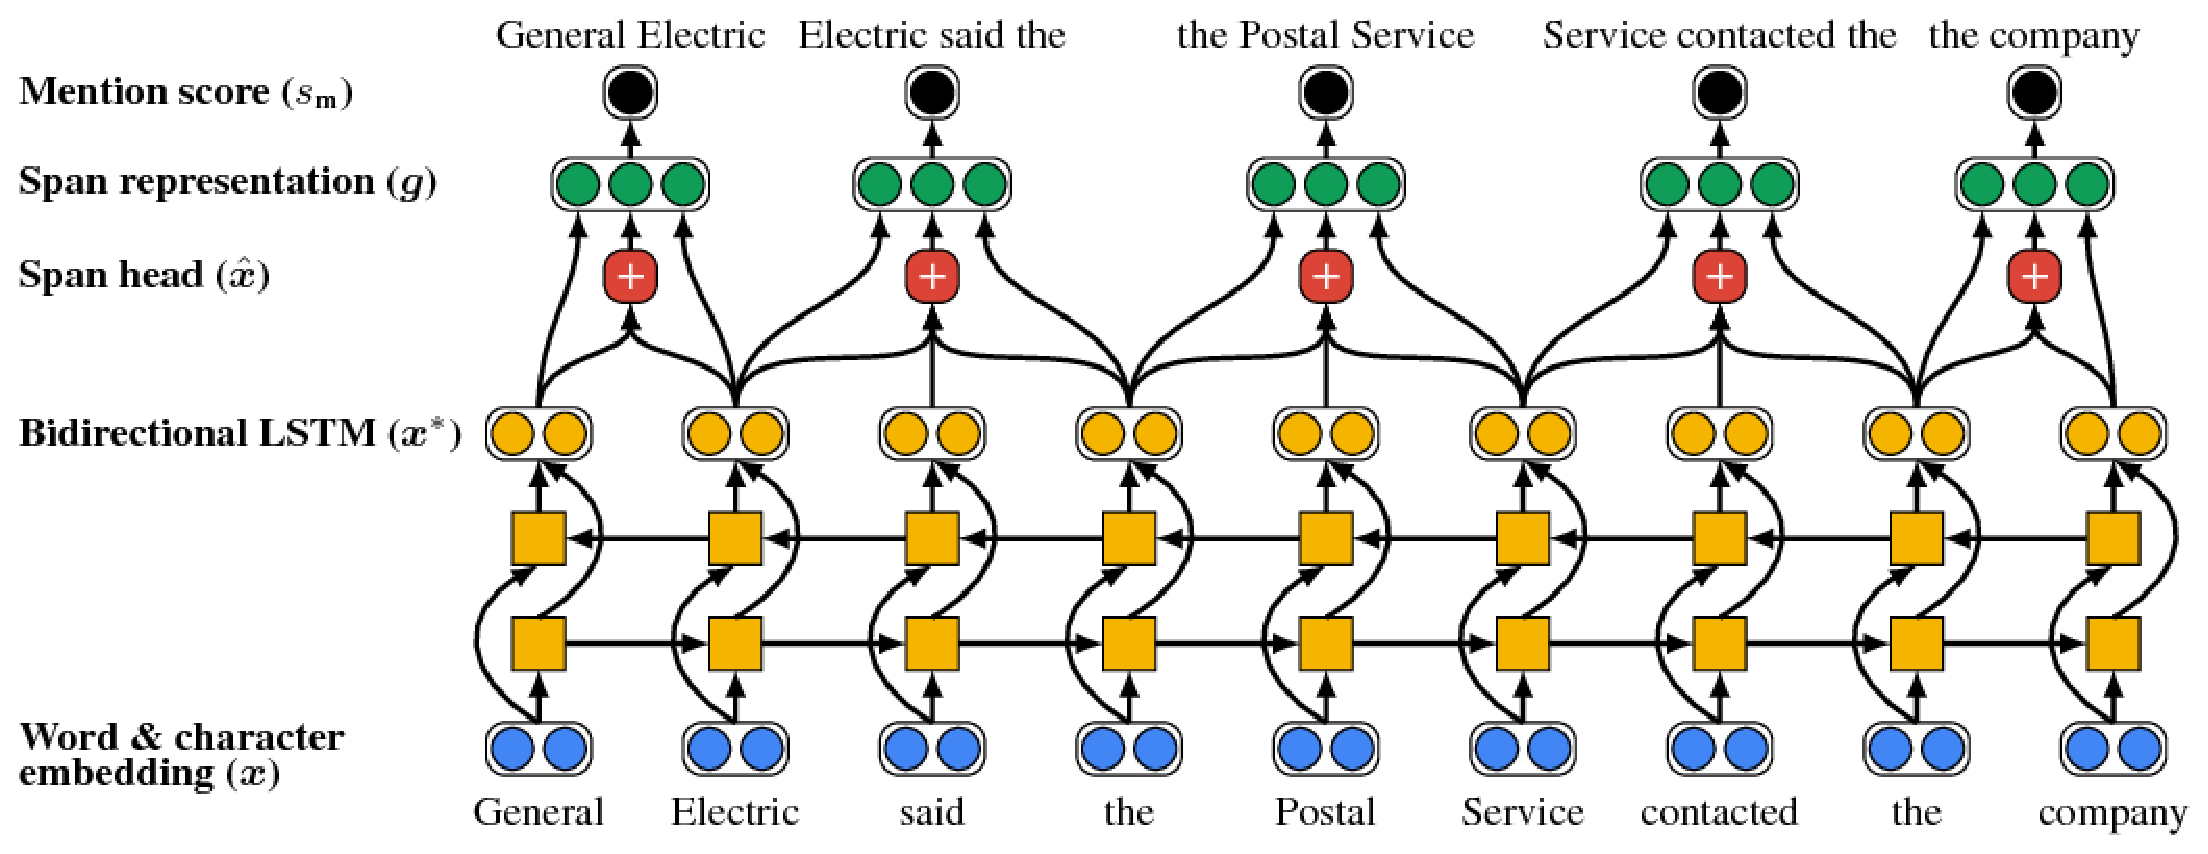
\includegraphics[width=\textwidth]{e2emodel.eps}
 % \caption{Figure 1: First step of the end-to-end coreference resolution model, which computes embedding representations of spans for scoring potential entity mentions. Low-scoring spans are pruned, so that only a manageable number of spans is considered for coreference decisions. In general, the model considers all possible spans up to a maximum width, but we depict here only a small subset. \parencite{lee2017end}}
 % \label{fig:e2emodel}
%\end{figure}

%\textcite{lee2017end} have proposed an span-ranking approach, which the authors describe as most similar to mention ranking, with reasoning over a larger space by detecting mentions and predicting coreference jointly in one end-to-end model. We will further refer to the model as \textit{e2e-coref}.


%The authors showed that from the space of all possible spans their model implicitly  learns to produce meaningful mention candidates. A head-finding attention mechanism also learns a task-specific preference for head words, which has a strong correlation with head-word definitions in rule-based systems.

%\begin{wrapfigure}{r}{0.5\textwidth} %this figure will be at the right
   % \centering
      %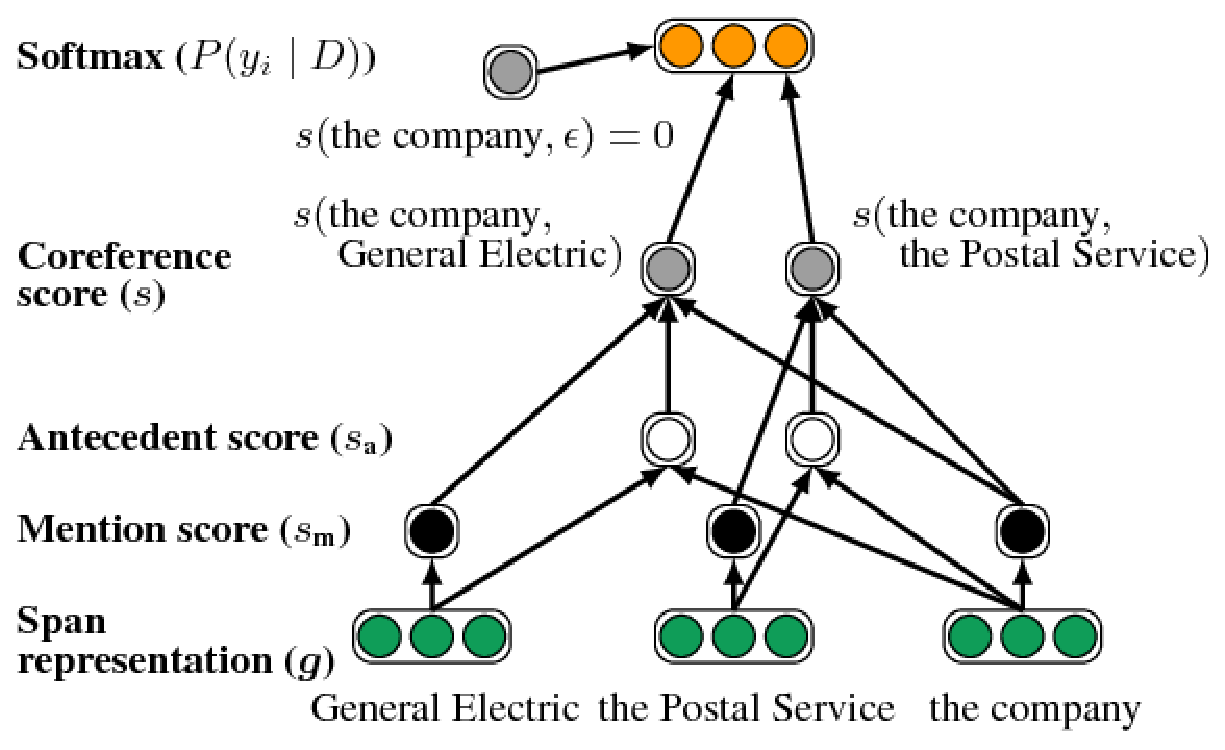
\includegraphics[width=0.5\textwidth]{e2e_extra_info.eps}
  %\caption{Second step of end-to-end model by \textcite{lee2017end}. Antecedent scores are computed from pairs of span representations. The final coreference score of a pair of spans is computed by summing the mention scores of both spans and their pairwise antecedent score.  }
  %\label{fig:e2e_extra_info}
%\end{wrapfigure}

%Building on to of the span-ranking neural architechture in \textcite{lee2017end}, \textcite{lee2018higher} proposed a model that captures higher order interactions
%between spans in predicted clusters. We will further refer to this model as \textit{c2f-coref}. It also alleviates the additional computational cost of higher-order inference due to a coarse-to-fine approach, which allows the model to at first compute a rough sketch of likely antecedents, and only at a later stage apply a more exhaustive inference. Hence, the coarse-to-fine approach expands the set of coreference links that the model is capable of learning. 

%To encode the span representations \textcite{lee2017end} use bidirectional LSTM \parencite{lstm} to encode the lexical information of the inside and
%outside of each span. \textcite{lee2018higher} additionaly use the newly published ELMo embedding representations by \textcite{peters2018elmo} at the input to the LSTMs.

%\textcite{joshi2019coref} took the architechture of \textcite{lee2018higher} and improved the performence of the model further by replacing the LSTM-based encoder with the BERT transformer \textcite{devlin2019bert}. We further refer to the model by \textcite{joshi2019coref} as \textit{bert-coref}.

%\textcite{devlin2019bert} made a significant break-through with their pre-trained BERT model. It can be finetuned with one additional output layer
%to create state-of-the-art models for a wide
%range of NLP tasks, such as question answering and language inference, without substantial taskspecific architecture modifications. BERT's training examples consist of 128 and 512 word pieces. Such passage-level training has been an important improvement over the previous methods. It helps the model learn dependencies over text sequences longer than one sentence, such as the previous state of the art model ELMo \parencite{peters2018elmo}. Two model sized have been presented by \textcite{devlin2019bert}:
%BERT-base(12 transformer blocks, hidden size 768, 12 self-attention heads, total Parameters=110M) and BERT-large (24 transformer blocks, hidden size 1024, 16 self-attention heads, total Parameters=340M).

%\begin{figure}[h]
  %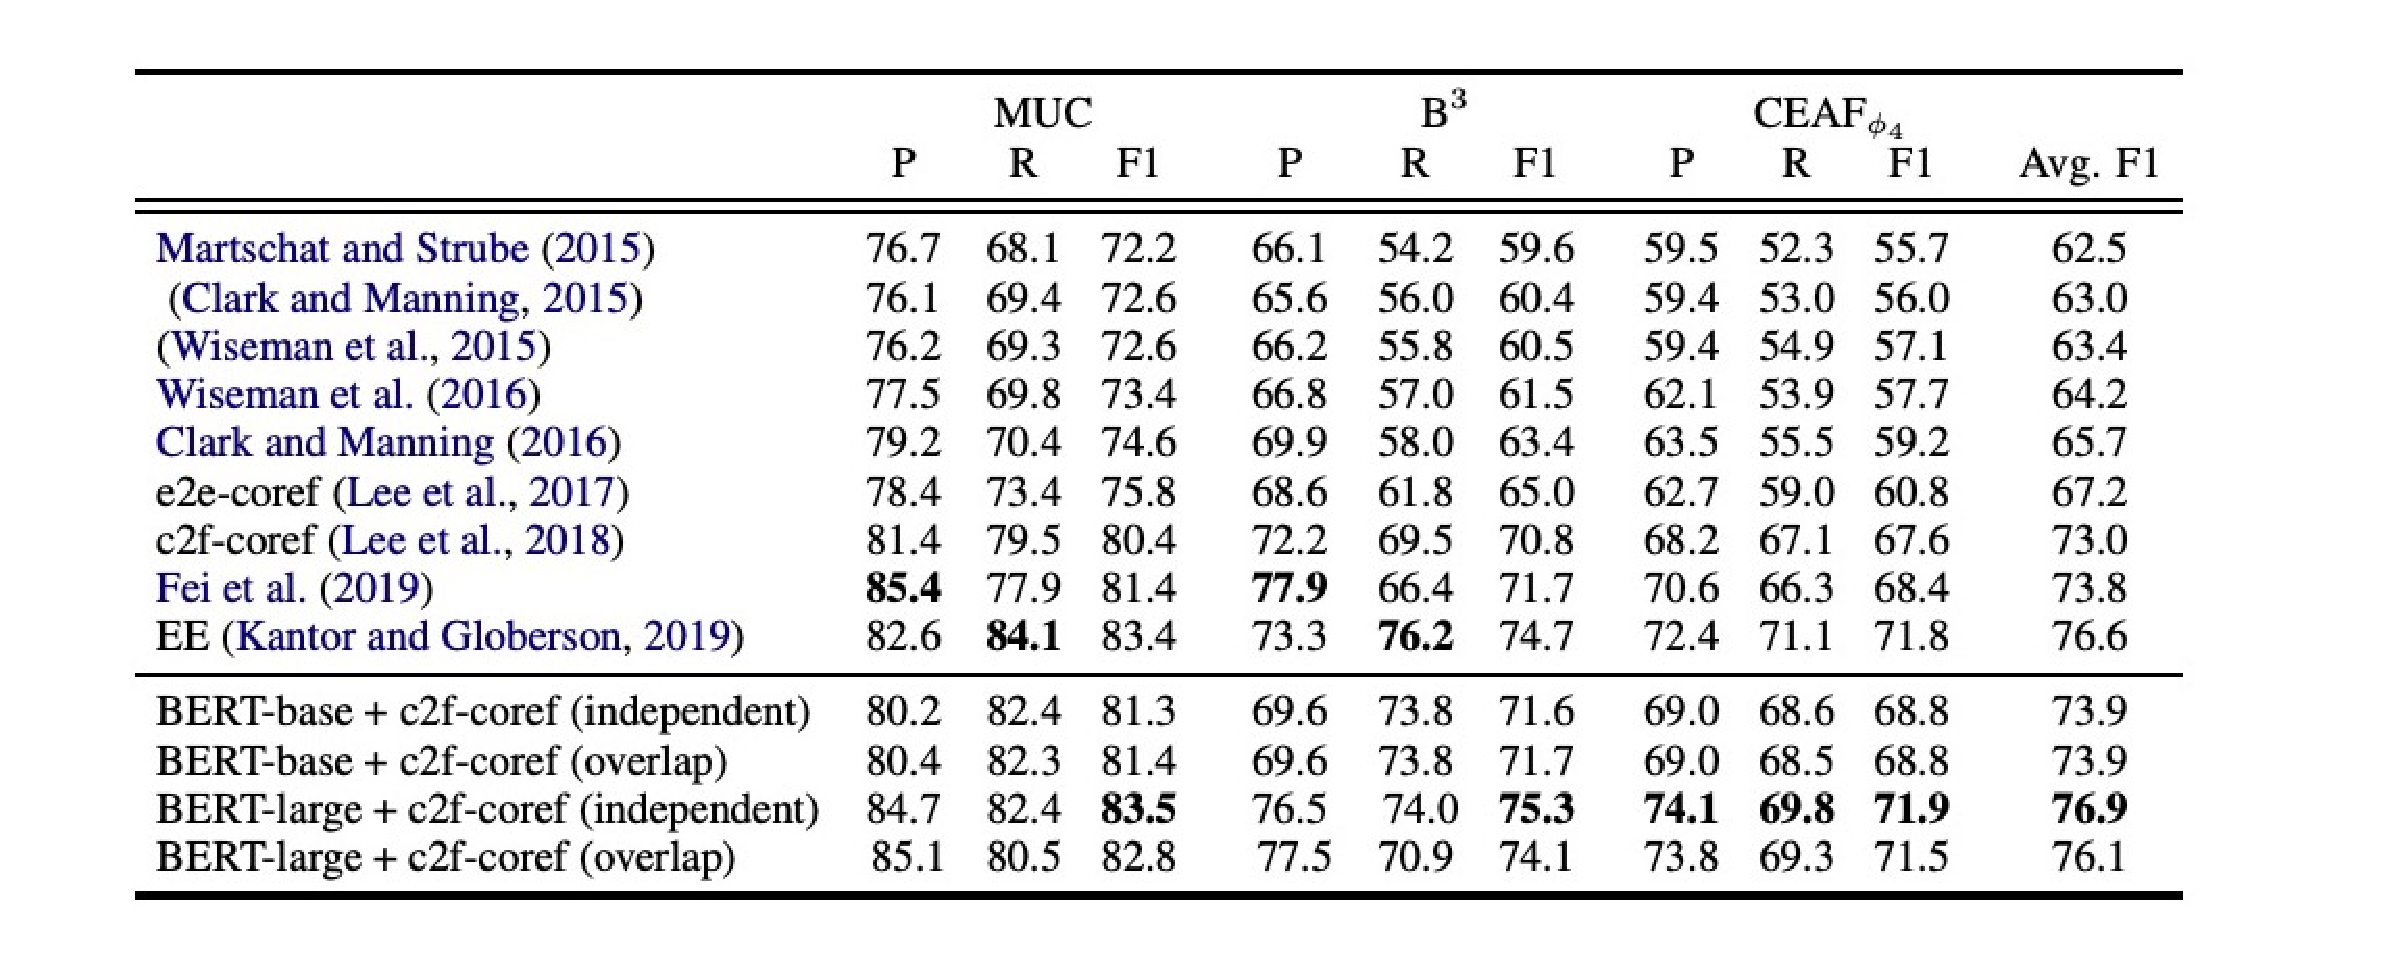
\includegraphics[width=\textwidth]{joshi_results.eps}
  %\caption{OntoNotes: BERT improves the c2f-coref model on English by 0.9\% and 3.9\% respectively for base and large variants. \parencite{joshi2019coref}}
  %\label{fig:joshiresults}
%\end{figure}

%\textcite{joshi2019coref} treat the first and last word-pieces in a mention (concatenated with the
%attended version of all word pieces in the span) as span representations. The researchers test both models with BERT-base and BERT-large transformers. With this change to the c2f-coref model the authors gain an additional 3.9\% improvement on the OntoNotes compared to the already high results of \textcite{lee2018higher}. A quantitative analysis is shown in  figure \ref{fig:joshiresults}. 
%A qualitative analysis done by the authors suggests that BERT-large (unlike BERT-base) is significantly better at distinguishing between related yet distinct entities or concepts.


\subsection{Probing Tasks}
% \textcite{liu2019linguistic}  Ling Knowledge and Transfer, Negative Samples, arc prediction task

% explain probing model in general, we are interested in particular in coref arc prediction
% describe work that has tried to probe coreference information in BERT
% clark et al show that given a coreferent mention BERT can predict a correct antecedent
% kantor and globerson, frozen bert
% xu and yang, GCN to capture syntax embeddings

% intro.. how analysis in NLP has been done....interpretability is an issue.. transition to probing model..


%Recently, there has been interesting work done to simplify state-of-the-art task-specific NLP models. 
% \textcite{liu2019linguistic} show evidence that frozen contextual represenations of word sequences fed into linear models can show similar levels of performance as state-of-the-art task-specific models on many NLP tasks.
%The authors use probing models, also known as auxiliary or diagnostic classifiers \parencite{shi2016string, kadar2017representation} to analyse the linguistic information within contextual word representations. To test how the probing model performs in comparison to ELMo, the authors tested the models on a coreference arc prediction task, where the model predicts whether two mentions corefer. The Ontonotes dataset was used. To train the probing model the authors generate negative examples, where mentions that do not corefer are fed into the probing model alongside the mentions that do corefer. In our work we will also build our experiments similar to coreference arc prediction tasks suggested by the authors.

%\textcite{tenney2019context} Probing Model
%\textcite{tenney2019context} introduced edge probing task design. For coreference resolution, the models had to determining whether two spans of tokens refer to the same entity. In order to investigate how good the contextual word representation models can model long-range dependencies, the authors used a fixed-width convolutional layer on top of the word representations to build spans of word pieces. The authors concluded that using the CNN layers on top of BERT-large pretarined model has performed particularly well on difficult semantic tasks, such as coreference resolution. Hence, in out work we will also follow the approach of the authors to construct our baseline. 
% and found that existing models trained on language modeling and translation produce strong representations for syntactic phenomena, but only offer comparably small improvements on semantic tasks over a non-contextual baseline. 

%tenney use span representation, but how will it perform using Lee's ?

Along with the rise of deep learning architectures across a plethora of NLP tasks, there is also some concern regarding its interpretability and whether if neural-based approach is able to capture linguistic concepts. The most common method to explore linguistic properties in neural network components is by using the hidden state activations to predict the property of interest, also known as "probing tasks" \parencite{conneau-etal-2018-cram} or "auxiliary prediction tasks" \parencite{auxilliarypredictiontasks}. \parencite{shi2016string} use the internal representations of LSTM encoder as an input to train logistic regression classifier that predicts various syntactic properties. \parencite{conneau-etal-2018-cram} study the linguistic properties of fixed-length sentence encoders with a bidirectional LSTM and gated convolutional networks.

\parencite{liu2019linguistic} explore representations produced by pretrained contextualizers and show that frozen contextual representations fed into linear models can show similar levels of performance as state-of-the-art task-specific models on many NLP tasks. They also introduced coreference arc prediction task, where linear models are used to predict whether if two mentions corefer. Concurrently, \parencite{tenney2019context} introduced edge probing framework, which focuses on linguistic analysis on sub-sentence level. Their approach uses a linear model with a projection layer and attention mechanism on top of frozen contextual vectors to predict linguistic properties. Our approach is most similar to \parencite{liu2019linguistic} and \parencite{tenney2019context}, but we use span representation by \parencite{lee2017end} and focus on examining coreference phenomena.



% describe approach to understand what neural network captures
% focus on span level 
\section{Overview of Span-Ranking Architecture}
% Move Lee 2017, Lee 2018, Joshi 2019 here, with a more in-depth explanation, separate it from Related Work
The first coreference resolution model that is trained in an end-to-end manner without relying on any syntactic parser or hand-engineered mention detector is introduced by \parencite{lee2017end}. To construct correct coreference clusters, the neural model learn to jointly model mention detection and coreference prediction using span-ranking approach.  With span-ranking approach, the model is able to consider all spans in a document up to a defined maximum length as a candidate mention and select the corresponding antecedent for each mention based on the antecedent distribution. We will further refer to the model as \textit{e2e-coref} in the paper.

The span-ranking architecture estimates the joint probability distribution of mention-spans that belong to the same cluster given the document, by calculating product of multinomials for each span:
\begin{align}
P(y_{1}, ..., y_{n}|D) &= \prod\limits_{i=1}^{N} P(y_{i}|D) \\
&= \prod\limits_{i=1}^{N} \frac{\text{exp}(s(i, y_{i}))}{\sum_{y' \in \mathcal{Y}(i)} \text{exp}(s(i, y'))}
\end{align}

where $s(i,j)$ is a pairwise score for a coreference link between span $i$ and span $j$ in document $D$. The coreference score is composed of three factors: (1) $s_{m}(i)$, mention score of $i$ (i.e. how possible is the span $i$ to be a mention), (2) $s_{m}(j)$, mention score of $j$ and (3) $s_{a}(i,j)$, joint score of $i$ and $j$ (i.e. assuming that $i$ and $j$ are both mentions, how possible that they both refer to the same entity), formulated as the following:
\begin{align}
s(i, j) = \begin{cases}
s_{m}(i) + s_{m}(j) + s_{a}(i, j) & j \neq \epsilon \\
0 & j = \epsilon
\end{cases}
\end{align} 

where $\epsilon$ is a dummy antecedent to represent that the span is not a mention or the case where it is a mention that coreferent with none of the previous mention span.

In this model, a bidirectional LSTM \parencite{lstm} is used to compute vector representations $\pmb{g}_{i}$ of each possible span $i$ from the word and character embeddings in the span. The word embeddings itself are a fixed concatenation of GloVe \parencite{pennington2014glove} and Turian embeddings \parencite{turian-etal-2010-word}. The character embeddings are learned using CNN, with three various window sizes. It also provide morphological information and allows the model to deal with rare words. The span representation $\pmb{g}_{i}$, which we will describe in detail in the following section, is then used to compute $s_{m}(i)$ and $s_{a}(i, j)$ via feed-forward neural networks as follows:
\begin{align}
s_{m}(i) &= \pmb{w}_{m} \cdot \text{FFNN}_{m}(\pmb{g}_{i}) \\
s_{a}(i, j) &= \pmb{w}_{a} \cdot \text{FFNN}_{a}([\pmb{g}_{i}, \pmb{g}_{j}, \pmb{g}_{i} \odot \pmb{g}_{j}, \phi(i, j)])
\end{align}

where $\odot$ denotes the Hadamard product between $\pmb{g}_{i}$ and $\pmb{g}_{j}$, and $\phi(i, j)$ is a feature vector that encodes speaker and genre information from the metadata and the distance between a pair of span. The final coreference score is computed through a two-stage beam search as the model complexity is quartic in terms of the document length. In the first phase, a beam of up to $\lambda T$ candidate mention spans are considered based on the highest mention scores $s_{m}(i)$, where $\lambda$ is a hyperparameter and $T$ is the document length. Afterwards, only the filtered mentions are used to compute the joint score $s_{a}(i, j)$ during both training and inference, with the limitation that only up to $K$ candidate antecedents that are considered for each mention.
% describe embeddings (glove, turian, etc) 
% describe encoder
% describe pruning for inference
% in case of emergency, insert figure.

% however quite costly, transition to higher order.
While the first order model proposed by \parencite{lee2017end} works quite well for coreference resolution, scoring only pairs of entity mentions means that previous coreference decisions are not taken into account when computing coreference decisions that occur afterwards. This drawback makes the model more susceptible to predicting clusters that are locally consistent but globally inconsistent. In an attempt to improve the weakness of this approach, \parencite{lee2018higher} proposed a model that captures higher-order interactions between mention spans in predicted coreference clusters. The model utilizes span-ranking architecture to refine existing span representations iteratively with the antecedent distribution as an attention mechanism. We will further refer to the model as \textit{c2f-coref} in the paper.

In order to refine the span representations, the higher-order model estimates the antecedent distributions $P_{n}(y_{i})$, which is obtained using the softmax function:
\begin{align}
P_{n}(y_{i}) = \frac{\text{exp}(s(\pmb{g}_{i}^{n}, \pmb{g}_{y_{i}}^{n}))}{\sum_{y \in \mathcal{Y}(i)} \text{exp}(s(\pmb{g}_{i}^{n}, \pmb{g}_{y}^{n}))}
\end{align}

where $s$ is the scoring function from \parencite{lee2017end}, $\pmb{g}_{i}^{n}$ is the representation for span $i$ at iteration $n$. The refined span representations also allow the model to iteratively refine $P_{n}(y_{i})$. Afterwards, the expectation of each span $i$ are computed by using the current antecedent distribution as the attention weight:
\begin{align}
\pmb{a}_{i}^{n} = \sum\limits_{y_{i} \in \mathcal{Y}(i)} P_{n}(y_{i}) \cdot \pmb{g}_{y_{i}}^{n}
\end{align}

where $\pmb{a}_{i}^{n}$ can be viewed as the expected antecedent representation. The span representation $\pmb{g}_{i}^{n}$ is updated with the expected antecedent representation $\pmb{a}_{i}^{n}$ using coupled forget and input gates formulated as the following:
\begin{align}
\pmb{f}_{i}^{n} &= \sigma(\textbf{W}_{f}[\pmb{g}_{i}^{n}, \pmb{a}_{i}^{n}]) \\
\pmb{g}_{i}^{n+1} &= \pmb{f}_{i}^{n} \odot \pmb{g}_{i}^{n} + (\mathbf{1} - \pmb{f}_{i}^{n}) \odot \pmb{a}_{i}^{n}
\end{align}

where $\pmb{f}_{i}^{n} \in [0,1]$ is a gate vector that controls whether to retain the information from the current span representation or to update the span representation with the expected antecedent. Altogether, this mechanism allows the model to compute the final antecedent distribution conditioned on up to $n$ other mention spans. 

To alleviate the additional computational cost of higher-order inference, \parencite{lee2018higher} also proposed a coarse-to-fine beam search, which does not establish an a priori maximum coreference distance. In order to prune potential mentions aggresively, the coreference score is reformulated as the following:
\begin{align}
s_{c}(i, j) &= \pmb{g}_{i}^{\top}\textbf{W}_{c}\, \pmb{g}_{j}\\
s(i, j) &= \begin{cases}
s_{m}(i) + s_{m}(j) + s_{a}(i, j) + s_{c}(i, j) & j \neq \epsilon \\
0 & j = \epsilon
\end{cases}
\end{align}

where $s_{c}(i, j)$ a bilinear scoring function to compute a rough sketch of possible antecedents. To obtain the coreference score, the model executes a three-stage beam search. At the first stage, a beam of up to $M$ candidate mention spans are considered based on the mention score $s_{m}(i)$. Afterwards,  approximation of pairwise coreference score is computed based on $s_{m}(i) + s_{m}(j) + s_{c}(i, j)$ to keep top $K$ candidate antecedents for each remaining mention spans. In the last phase, the final coreference score $s(i, j)$ is computed based on the surviving pairs of mention spans.
% describe latent antecedent trees in case of emergency

Recently, BERT \parencite{devlin2019bert} has achieved state-of-the-art results on a wide array of NLP tasks, such as question answering and natural language inference, without any substantial task-specific architecture modifications. \parencite{joshi2019coref} proposed to replace the bidirectional LSTM encoder in \textit{c2f-coref} with BERT transformers and fine-tune it on coreference resolution task. Although BERT improves the state-of-the-art results in other tasks significantly, coreference resolution still proves to be a challenging task, as BERT encoder offers only a marginal performance increase. Furthermore, the model still struggles in modeling pronouns and resolving cases where mention paraphrasing is required. We refer the model by \parencite{joshi2019coref} as \textit{BERT-coref}.


%describe iterative, enables later coreference decisions to softly condition on earlier coreference decisions.
%useELMO
%describe coarse to fine approximation
\section{Probing Mention-Span Representations}
% change section name to Probing Span Representations
% include overview of SOTA-architecture with BERT, preferably before the Probing Span Representations section
% Explain about Span Representations/Embeddings, especially regarding the features, define the span representations in SOTA

% Explain about the probing task, in this case Arc Prediction
% Explain about OntoNotes datasets, possibly can be moved to Experiments.
% Explain about probing model, possibly can be moved to Experiments. Explain also what is the input

\subsection{Span Representation}
\label{subsection:spanreps}

Span representation plays an important role in span-ranking model \parencite{lee2017end,lee2018higher}, since it is used to compute distribution over candidate antecedent spans. In order to be able to predict coreference relations accurately, span representation should also capture the information of the span's internal structure and its surrounding context. In our experiments, we use the span representation which is first proposed in \parencite{lee2017end}, but with BERT \parencite{devlin2019bert} instead of a LSTM-based encoder to encode lexical information of the span and its surrounding, following \parencite{joshi2019coref}. The span representation is a vector embeddings which consists of context-dependent boundary representations with attentional representation of the head words over the span. The boundary representations are composed of first and last word-pieces of the span itself. The head words are automatically learned using additive attention \parencite{bahdanau} over each word-pieces in the span:
\begin{align}
\alpha_{t} &= \pmb{w}_{\alpha} \cdot \text{FFNN}_{\alpha}(\pmb{x}_{t}^{*}) \\ 
a_{i,t} &=  \frac{exp(\alpha_{t})}{\sum\limits_{k=start(i)}^{end(i)} exp(\alpha_{k})} \\ 
\hat{\pmb{x}}_{i} &= \sum\limits_{t=start(i)}^{end(i)} a_{i,t} \cdot \pmb{x}_{t}
\end{align}

where $\hat{\pmb{x}}_{i}$ is a weighted vector representation of word-pieces for span $i$. This representation is augmented by a $\mathbb{R}^{d}$ feature vector which encodes the size of span $i$ with $d = 20$. The final representation $\pmb{g}_{i}$ for span $i$ is formulated as the following:
\begin{align}
\pmb{g}_{i} = [\pmb{x}_{start(i)}^{*}, \pmb{x}_{end(i)}^{*}, \hat{\pmb{x}}_{i}, \phi_{i}]
\end{align}  

where $\pmb{x}_{start(i)}^{*}$ and $\pmb{x}_{end(i)}^{*}$ are first and last word-pieces of the span, and $\phi_{i}$ is the span width embeddings.

\subsection{Coreference Arc Prediction}
\label{subsection:corefarc}

%Span representations will be then used as inputs for coreference arc prediction task \cite{liu2019linguistic}, where a probing model (in this case a simple FFNN) is used to predict coreference relations. The probing model is designed with limited capacity to focus on what information that can be extracted from the span representations. The probing model itself has a sigmoid output layer, which is trained to minimize binary cross entropy. Each negative samples (\textit{w\_entity}, \textit{wb}) will be generated for every positive samples (\textit{wa}, \textit{wb}) where \textit{wb} occurs after \textit{wa} and \textit{w\_entity} is a token that occurs before \textit{wb} and belong to a difference coreference cluster, to ensure a balanced data. By comparing the performance of the probing model using span representations, we can hypothesize to what extent that the proposed span representation in \textcite{joshi2019coref}  can capture coreference information. We will also experiment with mention span separation distance to see how the probing model performs and whether if there is a degradation of accuracy and F1 score of the probing model with distant spans.


% Tenney focus on span, Liu focus on CWR
We focus on coreference arc prediction task, which is a part of probing tasks suite for contextual word embeddings \parencite{liu2019linguistic, tenney2019context}. In this task, a probing model is trained to determine whether if two mentions refer to the same entity. As datasets for coreference resolution usually only contains annotations for corefering mentions, we produce negative samples following the approach by \parencite{liu2019linguistic}. For every pair of mentions $(w_{i}, w_{j})$, where they belong to the same coreference cluster and $w_{i}$ is an antecedent of $w_{j}$, we generate a negative example $(w_{random}, w_{j})$ where $w_{random}$ belongs to a different coreference cluster. This method ensures that the ratio between positive and negative examples is balanced. We also follow the approach of \parencite{tenney2019context} by using spans of word-pieces for mentions, as \parencite{liu2019linguistic}'s approach is limited on single-token mentions and therefore unable to fully exploit the information in the mention-span.


\subsection{Probing Model}
% add box to indicate frozen part!
\begin{figure}[ht]
  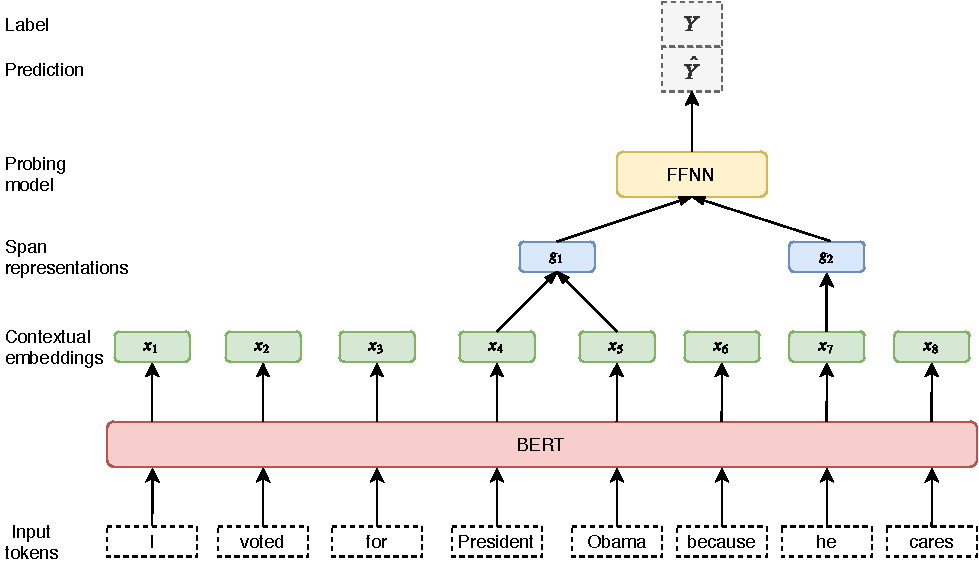
\includegraphics[width=\textwidth]{probing_model}
  \caption{Probing architecture for span representation. The feed-forward neural network is trained to extract information from the span representations $\pmb{g}_{1}$ and $\pmb{g}_{2}$, while all the parameters inside the dashed line are frozen. The example depicts a mention-pair, where $\pmb{g}_{1}$ corresponds to span representation of "President Obama", while $\pmb{g}_{2}$ corresponds to "he". We predict $\hat{Y}$ as positive for this example.}
  \label{fig:probing_model}
\end{figure}

Our probing model is a simple feed-forward neural network, which is designed with a limited capacity to focus on what information that can be extracted from the span representations.
As the input to our probing model, we take the span representation for pair of mention-spans $\pmb{g}_{1} = [\pmb{x}_{start(1)}^{*}, \pmb{x}_{end(1)}^{*}, \hat{\pmb{x}}_{1}, \phi_{1}]$ and $\pmb{g}_{2} = [\pmb{x}_{start(2)}^{*}, \pmb{x}_{end(2)}^{*}, \hat{\pmb{x}}_{2}, \phi_{2}]$, where both $\pmb{g}_{1}$ and $\pmb{g}_{2}$ are concatenated together and passed to the FFNN. The FFNN consists of a single hidden layer followed by a sigmoid output layer. The model is trained to minimize the binary cross-entropy with respect to the gold label $Y \in \{0,1\}$. The probing architecture is shown in Figure \ref{fig:probing_model}.
%Draw figure ffnn with positive and and negative examples ala tenney

% Explain using BERT-finetuned on OntoNotes and non-finetuned, base and large cased
We explore mention-span representations obtained from BERT. BERT \parencite{devlin2019bert} is a language representations model which uses deep Transformer architecture \parencite{transformers}, trained jointly with masked language model and next sentence prediction objective on BooksCorpus \parencite{bookscorpus} and English Wikipedia, with an approximate total of 3,300M tokens. It also enables significant improvement in many downstream tasks with relatively minimal task-specific fine-tuning. To study the quality of mention-span representations, we extract mention-span embeddings from BERT-base (12-layer Transformer, 768-hidden) and BERT-large (24-layer transformer, 1024-hidden). We also want to compare the effect of fine-tuning BERT-based models on the quality of span representations, therefore we use two variant of BERT models: a) fine-tuned on coreference resolution task and b) without any fine-tuning.



\section{Experiments}
% Explain that we do 2 experiments, first to see how the architectures improves span representation compared to non-finetuned BERT embeddings. Second one is to see long-range coreference phenomena.
% Explain pre-trained contextualized word embeddings that we used in the project, in this case BERT fine-tuned on OntoNotes and BERT which is not-fine tuned, use BERT-base and BERT-large cased, with 128 and 384 max segment length, because it is the best results. Independent variant
% Implementation and hyperparams
% Introduce baseline models here, also explain a bit regarding the attention..
% Explain how we see the long-range coference phenomena, with span separation distance.

% Move this to experiment
%We attempt to investigate 1) to what extent the span representations proposed using span embeddings with BERT \parencite{devlin2019bert} in \textcite{joshi2019coref} can encode coreference information, 2) and whether it is able to encode non-local coreference phenomena or is it just simply modeling local coreference.

%In order to analyse the first research question, we experiment with BERT-based span representations in \textit{bert-coref} model. The model is finetuned on OntoNotes. A single span represenattion for a mention consists of BERT embeddings for its first and last word-pieces concatenated with the attention version of all word pieces in the span. These span embeddings are a part of a larger \textit{bert-coref} model. \textcite{joshi2019coref} calculate several scores on top of span representations: mention score, antecedent score, and coreference score, which is then passed through a softmax layer. \ref{fig:e2e_extra_info} illustrates these additional layers. 

% move this part to analysis?
%For our research we refer to the work of \textcite{liu2019linguistic}. The research argue that frozen contextual represenations of word sequences fed into linear models can show similar levels of performance as state of the art task-specific models on many NLP tasks. We are interested in analysing how BERT span representations fed into a linear model will perform on a coreference task. For our experiments we will use a similar strategy as the coreference arc prediction task proposed by t\textcite{liu2019linguistic}.

%We extract the BERT span representations from a pipeline provided in a GitHub repository by \textcite{joshi2019coref} \footnote{\url{https://github.com/mandarjoshi90/coref}}. 

We attempt to investigate to what extent the proposed span representation using BERT embeddings and fine-tuned on corefence resolution task can encode coreference relations. We also want to answer whether if the span representation is able to encode long-range coreference phenomena effectively, or is it just simply modeling local coreference relation? Our experiments, which we describe below, are intended to analyze coreference information contained in the span representation used in the span-ranking model. 

\subsection{Dataset}
For our experiments, we use the coreference resolution annotation
from the CoNLL-2012 shared task based on the OntoNotes dataset \parencite{conll}. The dataset comprises of roughly one million words from various genre such as newswire, magazine articles, broadcast news, broadcast conversations, web data and conversational speech data, and the New Testament in English, which was splitted into 2802 training documents, 343 validation documents, and 348 test documents. On average, the training documents contain 454 words. The largest document contains a maximum of 4009 words. Beside entities, coreference is also annotated for mentions that refer to the same event (e.g. "The European economy \textbf{grew} rapidly over the past years, \textbf{this growth} helped raising...). The main evaluation of the dataset is the average F1 score of three metrics – $MUC$ \parencite{vilain-etal-1995-model}, $B^3$ \parencite{Bagga98algorithmsfor} and $CEAF_ \phi4$ \parencite{luo-2005-coreference}. Since OntoNotes only provide annotations for positive examples, we generate our own negative examples according to the aforementioned method (\S \ref{subsection:corefarc}). We also cast the original annotation provided in the dataset into JSON format in order to work with BERT-coref. 
% we work with jsonlines format by joshi, also mention the number of train, test, dev after casting?

\subsection{Implementation and Hyperparameters} 
%We extract the span representations from the coreference model by \textcite{joshi2019coref}. The model has been fine tuned on OntoNotes English data for 20 epochs using a dropout of 0.3, and learning rates of $1 * 10 ^{-5}$ and $2 * 10 ^{-4} $ with linear decay for the BERT parameters and the task parameters respectively. A batch size of 1 document has been used. 

We extend the original Tensorflow implementation of BERT-coref \footnote{\url{https://github.com/mandarjoshi90/coref}} in order to build our probing model with Keras frontend \parencite{chollet2015keras}. Our probing model are trained for 50 epochs, using early stopping with patience of 3 and batch size of 512. For optimization, we use Adam \parencite{adam} with a learning rate of 0.001. The weights of the probing model is initialized with Kaiming initialization \parencite{kaiming} and the size of the hidden layer is $d=1024$ with rectified linear units \parencite{relu}.

As mentioned previously, we use both original pre-trained BERT model without fine-tuning the encoder weights and BERT model that has been fine-tuned on coreference resolution task (i.e. on OntoNotes annotations). For fine-tuned BERT model, we take the models that yield the best performance on \parencite{joshi2019coref}, which were trained using 128 word-pieces for BERT-base and 384 word-pieces for BERT-large. The fine-tuned model was trained using splitted OntoNotes documents where each segment non-overlaps and fed as a separate instance. This is done as BERT can only accept sequences of at most 512 word-pieces and typically OntoNotes documents require multiple segments to be read entirely. In all of our experiments, we use the cased English BERT models.
% original BERT

\subsection{Baseline}
%As our baseline, w euse pre-trained BERT embeddings (not finetuned on OntoNotes) for all tokens within the mention span, which is then passed through a convolutional layer (with kernel width of 3 and 5) to incorporate the local context and followed by self-attention pooling operator to produce a fixed-length span representations. This is to model head words, inspired by approach from \textcite{tenney2019context}.

%max span width 30

%pooling is only within bounds of span, means that the only information our model can access about the rest of the sentence is provided by contextual embeddings of words within the span

% Describe span representation for baseline too! and padding part

As our baseline, we use span representations introduced in the edge probing framework \parencite{tenney2019context}. First of all, we take concatenated contextual embeddings for pair of mention-span $e^{(1)} = [x_{1}^{(1)}, x_{2}^{(1)}, x_{3}^{(1)}, ..., x_{n}^{(1)}]$ and $e^{(2)} = [x_{1}^{(2)}, x_{2}^{(2)}, x_{3}^{(2)}, ..., x_{n}^{(2)}]$ as inputs. We then project the concatenated contextual embeddings $e^{(1)}$ and $e^{(2)}$ to improve performance:
\begin{align}
e^{(i)} = Ae^{(i)} + b
\end{align}

where $i = (1,2)$, $A$ and $b$ are weights of the projection layer. The parameters in the projection layer are shared between representations $e^{(1)}$ and $e^{(2)}$. Afterwards, we apply self-attentional pooling operator in (\S \ref{subsection:spanreps}) over the projected representations to yield a fixed-length span representations. This also helps to model head words for each mention-span. These mention-span representations are then concatenated together and passed to the probing model to predict whether they corefer or not. It is important to note that the self-attention pooling is computed only using tokens within the boundary of the span. As a result, the model can only access information about the context surrounding the mention span through the contextual embeddings. We take the contextual embeddings from activations of non-finetuned BERT final layer, while freezing the encoder. The baseline probing architecture is depicted in Figure \ref{fig:baseline}. 

\begin{figure}[ht]
  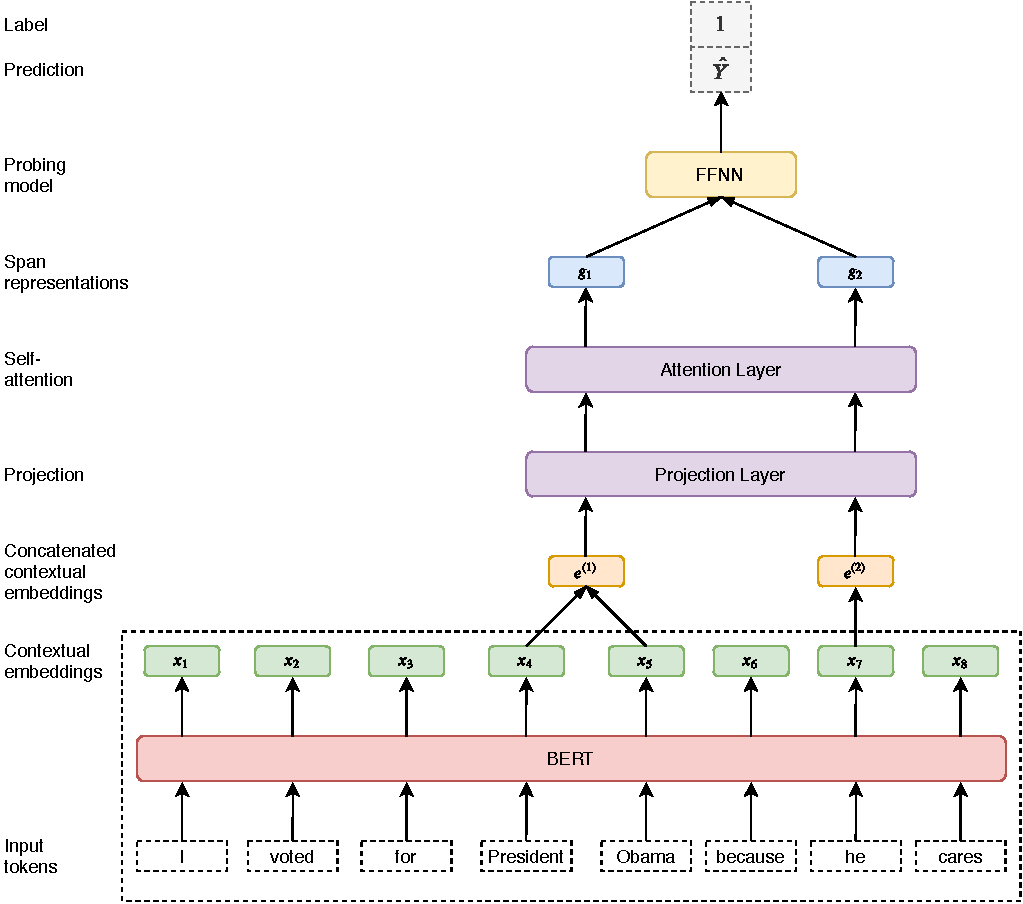
\includegraphics[width=\textwidth]{baseline_span}
  \caption{Probing architecture for baseline span representation. All parameters inside the dashed lines are frozen, while we train the feed-forward neural network to extract coreference information from the concatenated contextual embeddings $e^{(1)}$ and $e^{(2)}$. We used shared weights for both projection and self-attentional layer so that the model can learn the similarity between representation of mention-spans.}
  \label{fig:baseline} 
\end{figure}

%explain why the baseline is as it is
We compare the span representation used in the span-ranking model against the baseline, as it measures the performance that the probing model can achieve from the representation that is constructed from lexical priors alone, without any access to the local context within the mention-span. The resulting span representation have a dimension of $d = 768$ for BERT-base and $d = 1024$ for BERT-large.

\subsection{Long-range Coreference}
%In order to answer our second research question is whether the span representations encoded with a pre-trained BERT model simply modelling local coreference and will it be able to encode non-local coreference dependencies. In order to answer it, we bucket the test data into separate groups based on the the length of the coreference distance between the a mention and antecedent. We do separate qualitative and quantitative analysis on the buckets in order to analyse the differences in performance of our models based on how large the distance is. 

%does it capture local context? How does it perform on non-local context?
We want to understand better about the capability of the span representation from BERT encoder that is fine-tuned on coreference resolution task. Is it able to encode long-range coreference, or is it just simply modelling local coreference? We also want to answer how well does the model learn from local and long-range context within the mention-span. In order to answer both of these questions, we extend our baseline by introducing a convolutional layer to incorporate surrounding context and improves the baseline span representation, following \parencite{tenney2019context}. We replace the projection layer in our probing architecture with a fully-connected 1D CNN layer with a kernel width of 3 and 5, stride of 1 and same padding to properly include contextual embeddings at the beginning and end of the mention-span. This is equivalent to seeing $\pm$1 and $\pm$3 tokens around the center word respectively. We also initialize the weights of the CNN layer with Kaiming initialization \parencite{kaiming}. Using this extended probing architecture with CNN layer as another baseline, which we will refer to as CNN baseline in this paper, enables us to see the contribution of local and non-local context to the performance of the probing model. 

To investigate whether if the span representation is able to capture long-range coreference relation or not, we see how our probing model performs with various distance between mention-spans. We separate pair of mention-spans that appear in the OntoNotes test set into several buckets, based on the distance between last token of mention-span $w_{i}$ and first token of mention-span $w_{j}$, where $w_{j}$ occurs after $w_{i}$. Each bucket contains at least 50 examples of pair of mention-spans. 





% comparing to this see how well the model incorporate local and long-range context within a span to represent each word?

% Add this after discussing baseline and long-range coreference
% The resulting representations have a dimension of d=768 or 1024.


\section{Results}
\subsection{Comparison of Probing Models}
% Relate that it is possible to eliminate second step of the model? Seeing that probing model can be enough to predict coreference links?

% We generate representation from the encoder and train model to make predictions from those features alone. If a simple model can be trained to predict coreference from the span representation alone, we can reasonably conclude that the span representation encode this information

%learning task specific contextual features help to encode information for the span representation

% interesting to see that all baseline CNN and normal performs roughly the same
% CNN performs lower -> maybe because encoder is frozen

% explain how choice of span representation may help in encoding the informance required for the task.

% speculate BERT only improves a bit on semantic task, but a lot on syntactic task? (agree with tenney)

% explain how it is able to use local and non-local context

% interesting to see baseline still score so high, perhaps BERT architecture or MLM has something to do with this?

%should try using Joshi's span representation with original BERT weights, if still perform better, then it is the best span representation so far, if it is not, then fine-tuning is the important matter that encodes all the information. This opens up a venue to search for a better span representation.
We report the accuracies and F1 scores of our probing model with span representations constructed with BERT encoder. Table \ref{table:spanscore} compares the performance of probing model using span representations finetuned on OntoNotes dataset against baseline span representation and CNN baseline that utilize non-finetuned BERT encoder. Using a simple linear probing model, we demonstrate that span representation in BERT-coref encodes a significant amount of coreference information, as we are able to train the probing model to predict whether a pair of mention spans corefer or not based on their span representations alone. Both BERT-base c2f and BERT-large c2f consistently scores above 90\% (accuracy and F1 score) on OntoNotes test set. 

\begin{table}[ht]
\captionsetup{singlelinecheck = false, justification=justified}
\setlength\tabcolsep{0pt} % let LaTeX figure out amount of inter-column whitespace
\label{turns}
\begin{tabular*}{\textwidth}{@{\extracolsep{\fill}} l *{3}{d{2.4}} }
\toprule
 & \multicolumn{1}{c}{Accuracy} & \multicolumn{1}{c}{F1 Score}\\
\midrule
\midrule
BERT-base c2f (cased, fine-tuned)     & 92.93 & 93.02 \\
BERT-large c2f (cased, fine-tuned)    & 93.65\ast & 93.68\ast \\
\midrule
BERT-base CNN (cased, original, kernel=3)  & 89.51 & 89.91  \\
BERT-base CNN (cased, original, kernel=5)  & 89.04 & 89.28 \\
BERT-large CNN (cased, original, kernel=3) & 90.27 & 90.35 \\
BERT-large CNN (cased, original, kernel=5) & 88.09 & 88.28 \\
\midrule
BERT-base (cased, original) baseline		 & 90.37 & 90.65 \\
BERT-large (cased, original) baseline     & 91.47 & 91.69 \\
\bottomrule
\end{tabular*}
\caption{Comparison of the probing model's performance with various mention-span representations evaluated on OntoNotes test set. Asterisk denotes the best performance on each metric. BERT-large c2f improves the accuracy and F1 score over the probing baseline by 3.28\% and 3.03\% for the base variant, while for BERT-large baseline, the improvements are 2.18\% and 1.99\% respectively.}
\label{table:spanscore}
\end{table}
%include score in Liu's as rough comparison? Although it is not directly comparable?

We observe that both BERT-base c2f and BERT-large c2f performs better in predicting coreference arc between a pair of mention-spans compared to their respective baseline (by 2.37 points for accuracy and 2.18 F1 points on average). We find that although training the contextual probing model to learn contextual features for coreference arc prediction helps in encoding the necessary coreference information into the baseline span representation, it still cannot outperform the probing model that utilizes span representation in BERT-coref. This might be caused by better coreference-related features that is learned by BERT encoder when it is fine-tuned on OntoNotes.

We find that fine-tuning the span representation on coreference resolution task helps to encode local and long-range context inside the mention-span efficiently. This can be observed from the performance of CNN baseline, where the probing model is trained using 1D CNN layer with kernel width of 3 and 5 to allow us to see contribution of local and long-range dependencies, but ultimately still perform lower compared to BERT-coref. Surprisingly, our baseline span representation which is constructed from only lexical prior performs better compared to the CNN baseline span representation on both metrics. We attribute this due to our decision of taking contextual embeddings from the final layer of pre-trained BERT, as most transferrable representations from contextual encoders trained with language modeling objective tend to occur in the intermediate layers, and that the topmost layers might be overly specialized for next-word prediction \parencite{liu2019linguistic,peters2018elmo,peters-etal-2018-dissecting,blevins-etal-2018-deep,devlin2019bert}. This may cause the CNN layer to learn suboptimal representations from the mention-span.
%span ends span beginning

\subsection{Ablations}
To find out the importance of each component in BERT-coref span representations, we do ablation study on each part of the representation and report the accuracy and F1 score of the probing model on the test set of the data, which is depicted on Table \ref{table:ablation}. The head-finding attention mechanism is crucial for coreference-arc prediction, as it contributes the highest to the final result with 0.98 and 0.95 points for accuracy and F1 score on average, respectively. This is consistent with previous findings from \parencite{lee2017end}, where attention mechanism is shown to be able to learn representation that is important for coreference. We also observe that span-width embeddings play an important role in determining coreference relation, seeing that without them the performance degrades on average by 0.4 and 0.37 for accuracy and F1. Contrary to the head-finding attention and span-width embeddings, boundary representations did not contribute much to the model's performance. We hypothesize that although boundary representations encode rich amount of information for coreference resolution, it is not significant for coreference arc prediction, as the model does not have to predict distribution over possible spans.

\begin{table}[ht]
\captionsetup{singlelinecheck = false, justification=justified}
\setlength\tabcolsep{0pt} % let LaTeX figure out amount of inter-column whitespace
\label{turns}
\begin{tabular*}{\textwidth}{@{\extracolsep{\fill}} l *{4}{d{1.2}} }
\toprule
 & \multicolumn{1}{c}{Accuracy} & \multicolumn{1}{c}{F1 Score} & \multicolumn{1}{c}{$\Delta \text{Accuracy}$ } & \multicolumn{1}{c}{$\Delta \text{F1 Score}$}\\
\midrule
\midrule
BERT-base c2f (cased, fine-tuned)     & 92.93 & 93.02 \\
- boundary representations 				  & 92.88 & 92.96 & -0.05 & -0.06\\
- head-finding attention   					  & 92.05 & 92.16 & -0.88 & -0.86 \\
- span-width embeddings 				  & 92.46 & 92.56 & -0.47 & -0.46 \\
\midrule
BERT-large c2f (cased, fine-tuned)    & 93.65 & 93.68 \\
- boundary representations 				  & 93.47 & 93.49  & -0.18 & -0.19\\
- head-finding attention   					  & 92.57 & 92.65 & -1.08 & -1.03\\
- span-width embeddings 				  & 93.32 & 93.41 & -0.33 & -0.27\\
\bottomrule
\end{tabular*}
\caption{Comparison of the probing model on OntoNotes test set with various components removed. The head-finding attention and span-width embeddings contribute significantly to the performance of the probing model.}
\label{table:ablation}
\end{table}

\subsection{Encoding Long-range Coreference}

We compare how our probing model performs with various span separation distance in order to explore whether if the span-representation is able to encode long-range coreference or not. Figure \ref{fig:longrange_result} depicts F1 score as a function of the distance of wordpiece tokens between a pair of mention-spans. Although performance with BERT models degrade with larger distance over pair of mention-span, the span representation in BERT-coref holds up better in general compared to the baseline or CNN baseline. The BERT-base variant experiences minor degradation in performance to 5 points when $d=125$ tokens, while for BERT-large, the F1 score dropped only by 7 points between $d=0$ tokens and $d=250$ tokens, which suggests that the depth of Transformer layer helps to encode long-range coreference. However, we lack sufficient evidence to suggest that the span representation is able to encode long-range coreference relation efficiently, seeing that although already the encoder has been fine-tuned on OntoNotes, the model still cannot perform consistently across distant spans, with the lowest F1 score of 0.67 and 0.75 points for BERT-base and BERT-large respectively, when $d=451$ to $475$ tokens.
\begin{figure}[ht]
\subfloat[]{\label{subfig:bertbase}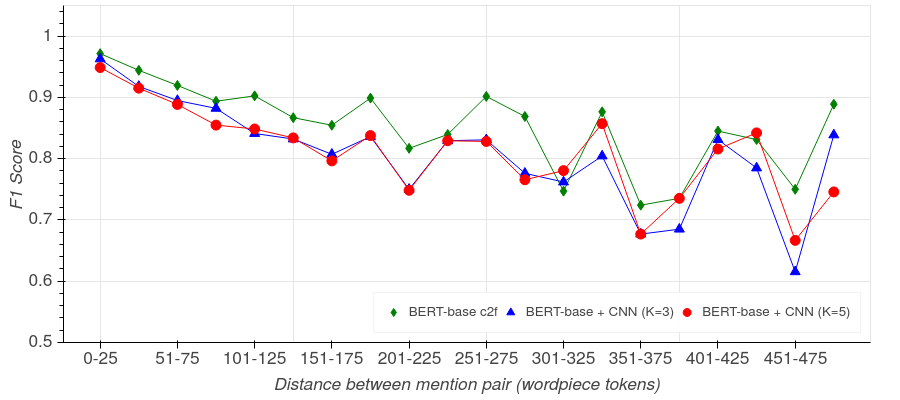
\includegraphics[clip, width=\textwidth]{long_range_bert_base}} \\
\subfloat[]{\label{subfig:bertlarge}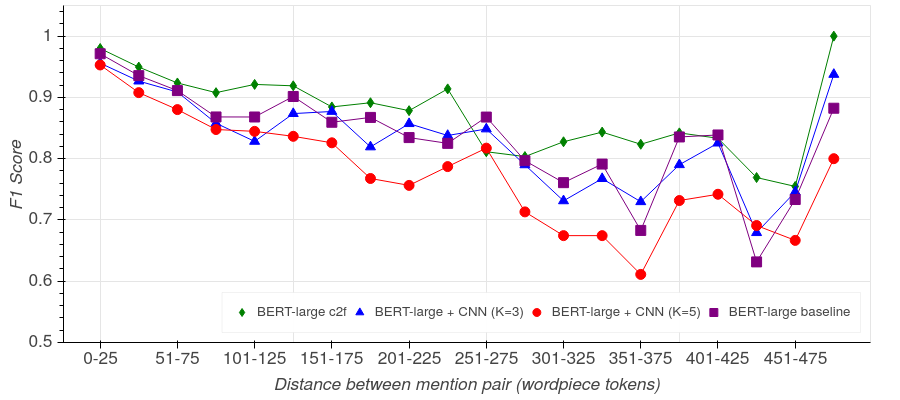
\includegraphics[clip, width=\textwidth]{long_range_bert_large}}
  \caption{F1 score of probing model as a function of separating distance between two mention-spans with BERT-base (\ref{subfig:bertbase}) and BERT-large (\ref{subfig:bertlarge}) on test set. The performance with either BERT-base or BERT-large tend to fall off as distance between wordpiece token increases.}
  \label{fig:longrange_result} 
\end{figure}
\section{Discussion}


\subsection{Design of Qualitative Analysis}

% confusion matric bert-base
\begin{table}[ht]
\captionsetup{singlelinecheck = false, justification=justified}
\setlength\tabcolsep{0pt} % let LaTeX figure out amount of inter-column whitespace
\label{turns}
\begin{tabular*}{0.8\textwidth}{@{\extracolsep{\fill}} l *{4}{d{1.2}} }
\toprule
  \multicolumn{1}{c}{} & \multicolumn{1}{c}{True Coreferent} & \multicolumn{1}{c}{True Non-Coreferent} &  \multicolumn{1}{c}{Precision} \\ 
  \midrule
  \midrule
\makecell[l]{Predicted \\ Coreferent}  & 
\multicolumn{1}{c}{\makecell{575 \\ True Positives}} & \multicolumn{1}{c}{\makecell{51 \\ False Positives}} & 0.92 \\
\midrule 
\makecell[l]{Predicted \\ Non-Coreferent} & 
\multicolumn{1}{c}{\makecell{42 \\ False Negatives}} & \multicolumn{1}{c}{\makecell{580 \\ True Negatives}} & \\
\midrule
Recall & 0.93 & & \\
\bottomrule
\end{tabular*}
\caption{Confusion Matrix for BERT-base c2f. Subset Size is 1250 data points.}
\label{table:confusion-matrix-base}
\end{table}

% confusion matric bert-large
\begin{table}[ht]
\captionsetup{singlelinecheck = false, justification=justified}
\setlength\tabcolsep{0pt} % let LaTeX figure out amount of inter-column whitespace
\label{turns}
\begin{tabular*}{0.8\textwidth}{@{\extracolsep{\fill}} l *{4}{d{1.2}} }
\toprule
  \multicolumn{1}{c}{} & \multicolumn{1}{c}{\makecell{True \\ Coreferent}} & \multicolumn{1}{c}{\makecell{True \\ Non-Coreferent}} & \multicolumn{1}{c}{Precision} \\ 
 \midrule
 \midrule
 \makecell[l]{Predicted \\ Coreferent}  & 
\multicolumn{1}{c}{\makecell{576 \\True Positives}} & \multicolumn{1}{c}{\makecell{40 \\ False Positives}} & 0.93 \\
\midrule 
\makecell[l]{Predicted \\ Non-Coreferent} & 
\multicolumn{1}{c}{\makecell{44 \\ False Negatives}} & \multicolumn{1}{c}{\makecell{588 \\ True Negatives}} & \\
\midrule
Recall & 0.93 & & \\
\bottomrule
\end{tabular*}
\caption{Confusion Matrix for BERT-large c2f. Subset Size is 1250 data points.}
\label{table:confusion-matrix-large}
\end{table}

Our aim is to present qualitative error analysis for predicted coreference between mention-pairs. We identify and characterize a set of challenging errors common to state-of-the-art systems dealing with coreference resolution in English. Such quialitative analysis enables us to detect patterns in errors that our system produces and to discuss underlying reasons for such errors. As true positives we treat the pair of one mention and another mention belonging to the same coreference chain which matches the corresponding mention in the gold standard. 

We conducted our error analysis on 4 models: BERT-base c2f (cased, fine-tuned), BERT-large c2f (cased, fine-tuned), BERT-base (cased, original) baseline, and BERT-large (cased, original) baseline. We used a subsample of 100 coreference clusters from the Ontonotes test dataset. We divide errors into the following categories: \textit{Related Entities, Lexical, Pronouns, Gender, Mention Paraphrasing, Conversation,} and \textit{Misc}. Although \textit{Gender} can be considered a subcategory of \textit{Pronouns}, the decision to separate it is motivated by the curiosity to find out whether gender bias is present in the models. 


% joshi 0-25 error analysis

\begin{table}[ht]
\captionsetup{singlelinecheck = false, justification=justified}
\setlength\tabcolsep{0pt} % let LaTeX figure out amount of inter-column whitespace
\label{turns}
\begin{tabular*}{\textwidth}{@{\extracolsep{\fill}} l *{4}{d{1.2}} }
\toprule
\multicolumn{1}{c}{Category} & \multicolumn{1}{c}{Snippet} & \multicolumn{1}{c}{base c2f} & \multicolumn{1}{c}{large c2f}  \\
\midrule
\midrule
\makecell[l]{Similar \\ Word Forms} & \multicolumn{1}{l}{\makecell[l]{... in some of the questioning eh of \textit{Miller}, I think ... \\ you have \textit{Judy Miller} there ( 13 )  \\  \textit{Director Men Xianlong, Mr. Meng Xianlong, of the} \\ \textit{Command Center of the Beijing Municipal Traffic} \\ \textit{Administration} ... hear what \textit{Director Meng said} ... ( 7 ) }} & 3 & 0 \\
\midrule
\makecell[l]{Anaphora} & \multicolumn{1}{l}{\makecell[l]{... it was very prompt with\textit{ traffic management and} \\ \textit{emergency repair} ... ah, because \textit{it} involved various ( 5 ) \\ ... \textit{the number of science and technology consulting} \\ \textit{enterprises}  ... more than double of \textit{that} ... ( 10 ) }} & 9 & 5 \\
\midrule
Gender & \multicolumn{1}{l}{\makecell[l]{none}} & 0 & 0 \\
\midrule
\makecell[l]{Mention \\ Paraphrasing} & \multicolumn{1}{l}{\makecell[l]{When someone sews a patch over \textbf{a hole in an old coat},\\  they ... If they do, \textbf{the patch} will shrink ( 22 )}} & 1 & 1 \\
\midrule
\makecell[l]{Temporal \\ and Spacial} &  \multicolumn{1}{l}{\makecell[l]{... people from economic circles, who even predicted that \\ in \textit{1998} ... They pointed out that, \textit{this year}, except ... ( 13 ) \\ ... \textbf{the Jiang-Huai area} ... experience continuous rainfall. \\ ... \textbf{the Huang-Huai area} will bid ... ( 23 ) }} & 1 & 2 \\
\midrule
Total &  & 14 & 8 \\
\bottomrule
\end{tabular*}
\caption{Error Analysis of BERT-base c2f and BERT-large c2f models for examples with short-range coreference (0-25 tokens apart). False positives are denoted \textbf{bold}, false negatives -- \textit{cursive}. }
\label{table:error-0-25}
\end{table}

In the table: bold are false positives, cursive are false negatives.

Our hypothesis is that mentions that are separated by a large distance will have a higher error rate in all categories. 

The most difficult for all models is ... \todo{add this}. There is a tendency for all systems to ... \todo{add this}. The least problematic category for all models is... 

% subsections for error categories
\subsection{Similar Word Forms} 
The word forms of the two mentions are similar, or the same graphems appear in both mentions, but they refer to different entities.

\subsection{Anaphora}

Pronouns coreference spanning over 100 tokens is intrinsically difficult, even for a human. The model predicts pronouns relating to a mention 200 tokens in distance. 

Agreement is good even when predicting oven 200 words. - Them == her colleagues guesses correctly

\subsection{Gender}
Usually in context of a gender pronoun relating to a name of a person.
no problems with common names. 
In the analysed subsample only one source of errors -- \textbf{Scooter Libby} is predicted to corefer with \textit{she}. Interestingly, a male name is considered to be female and not the other way around, as one would expect. 


\subsection{Mention Paraphrasing} Error in failing to label two mentions as referring to the same entity on one hand and labelling two distinct mentions as coreferent on the other hand.

Goods and Intellectual property Rights are deemed coreferent by joshi base: legally speaking different things. Might occur in similar laws.

Jesus and Young Man. Part of the dialog between Jesus and a young man.


\subsection{Temporal and Spacial Agreement}
Mention paraphrasing with reference to a specific date (e.g. January 3 and yesterday) and a specific spacial areas (two Chinese provinces).

1996 and 1997 are labeled as coreferent by joshi's base model. Or this year and 1994. This is a mistake that a human will likely not do.

% joshi 26-100 error analysis
\begin{table}[ht]
\captionsetup{singlelinecheck = false, justification=justified}
\setlength\tabcolsep{0pt} % let LaTeX figure out amount of inter-column whitespace
\label{turns}
\begin{tabular*}{\textwidth}{@{\extracolsep{\fill}} l *{4}{d{1.2}} }
\toprule
\multicolumn{1}{c}{Category} & \multicolumn{1}{c}{Snippet} & \multicolumn{1}{c}{base c2f} & \multicolumn{1}{c}{large c2f}  \\
\midrule
\midrule
\makecell[l]{Similar \\ Word Forms} & \multicolumn{1}{l}{\makecell[l]{... the big news for me was Miller \textbf{recounting} what ...\\  Tate by the way tells the Times that that \textbf{account} is false ( 76 ) \\ ... this is the Dick Cheney aide she \textbf{agreed} to refer ... \\ I think the \textbf{agreement} was strange ( 85 ) }} & 3 & 5 \\
\midrule
\makecell[l]{Anaphora} & \multicolumn{1}{l}{\makecell[l]{Actually, this morning, \textit{some listeners}, ah, happen to tell ... \\ a lot of \textit{them} as well as a lot of our friends ... ( 44 ) \\ ...the reactions of citizens. -- an SMS. \textbf{I} saw it ... \\ took the subway here. Do \textbf{you} think that ... ( 96 ) }} & 15 & 14 \\
\midrule
Gender & \multicolumn{1}{l}{\makecell[l]{... killed a piece written by a reporter about\textbf{ Scooter Libby} ... \\ They didn' t say that you know until \textbf{she} walked out ( 58 )}} & 0 & 1 \\
\midrule
\makecell[l]{Mention \\ Paraphrasing} & \multicolumn{1}{l}{\makecell[l]{... when importing and exporting \textbf{goods} ... \\ The owners of \textbf{intellectual property rights} who ... ( 77 ) \\ ... as many as three times the role of Valerie Plame ... \\ millions of dollars in legal fees in \textbf{Miss Miller's} case. ( 54 ) }} & 8 & 4 \\
\midrule
\makecell[l]{Temporal \\ and Spacial} &  \multicolumn{1}{l}{\makecell[l]{... the Huang-Huai area through \textbf{southern North China} ... \\ there will also be less snow in \textbf{Northwest China} ( 80 ) \\ ... some areas of South China, \textbf{Southwest China}, and ... \\ southern North China and \textbf{the Huang-Huai area} ... ( 80 ) }} & 2 & 2 \\
\midrule
Total &  & 28 & 26 \\
\bottomrule
\end{tabular*}
\caption{Error Analysis of BERT-base c2f and BERT-large c2f models for examples with middle-range coreference (26-100 tokens apart). False positives are denoted \textbf{bold}, false negatives -- \textit{cursive}. }
\label{table:error-26-100}
\end{table}


The most difficult for 


% \begin{itemize}
% \item long long analysis of what we've seen
% \item generalisations, parallels
% \item what do this results tell us about coref and nlp in general
% \item discussion of why they are the way the are
% \end{itemize}

\subsection{Other Languages}

The results we introduced in this paper has been tested solely on an English corpus.
Hence, the high results may be a phenomena particular to this language. For morphologically or syntactically complex languages the models would have struggled more. A benefit of using neural models for coreference resolution is their ability to use contextualized word embeddings to capture similarity between words, a property that many traditional feature-based models lack. However, a similar analysis should be done for other languages before one can generalize that machine-learning based models outperform rule-based models universally. % maybe it's more relevant in the conclusion A: I rewrote it. what about now?

% over 100
\begin{table}[ht]
\captionsetup{singlelinecheck = false, justification=justified}
\setlength\tabcolsep{0pt} % let LaTeX figure out amount of inter-column whitespace
\label{turns}
\begin{tabular*}{\textwidth}{@{\extracolsep{\fill}} l *{4}{d{1.2}} }
\toprule
\multicolumn{1}{c}{Category} & \multicolumn{1}{c}{Snippet} & \multicolumn{1}{c}{base c2f} & \multicolumn{1}{c}{large c2f}  \\
\midrule
\midrule
\makecell[l]{Similar \\ Word Forms} & \multicolumn{1}{l}{\makecell[l]{... they contacted \textbf{Clinton' s office back} in ... \\ the first time that the \textbf{Clinton forces} learned about ... ( 370 ) \\ 
... of the different departments of \textit{Beijing Municipality} ... \\ received this order from the \textit{municipal government}( 200 ) }} & 11 & 8 \\
\midrule
\makecell[l]{Anaphora} & \multicolumn{1}{l}{\makecell[l]{ ... took so long is that not only was \textbf{she} negotiating ... \\ And on that point \textbf{Arianna} on that ... ( 180 ) \\ ... the news on the day of \textit{the accident} ... \\ instead of the east and \textit{it} did not ( 277 ) }} & 23 & 22 \\
\midrule
Gender & \multicolumn{1}{l}{\makecell[l]{... not accept the waiver of confidentiality that Scooter Libby \\ offered ... her notes while they were defending her ( 1141 )}} & 0 & 1 \\
\midrule
\makecell[l]{Mention \\ Paraphrasing} & \multicolumn{1}{l}{\makecell[l]{ ... but first \textbf{Judy Miller and the New York Times} finally ... \\ in covering the controversy \textbf{the editors} killed ... ( 226 ) \\ ...  read a statement from \textbf{a Sixty Minutes spokesman} ... \\ When \textbf{Mister Carson the representative} spoke ... ( 241 ) 
.}} & 11 & 14 \\
\midrule
\makecell[l]{Temporal \\ and Spacial} &  \multicolumn{1}{l}{\makecell[l]{ ... and only 582 million US dollars \textbf{last year}... \\ momentum can not be restrained, \textbf{this year} ... ( 379 ) \\ 
... News Agency, the UN, \textit{February 13th}, Today ... \\  multi-national forces on \textit{the 13th} at 4 ( 153 ) 
}} & 6 & 5 \\
\midrule
Total &  & 51 & 50 \\
\bottomrule
\end{tabular*}
\caption{Error Analysis of BERT-base c2f and BERT-large c2f models for examples with long-range coreference (over 100 tokens apart). False positives are denoted \textbf{bold}, false negatives -- \textit{cursive}. }
\label{table:error-over-100}
\end{table}


\section{Conclusion and Future Work}

\begin{itemize}
\item so what have we learned about coref in general and local dependencies in particular
\item everything we don't have the time for
\item mention other corpora that could be used for finetuning (Winogrande, GAP...)
\item apply roberta, spanbert (sota result, architecture still use c2f)
\item try building span representations from intermediate layers, use scalar mixing
\item comparing attention head of Joshi's and
\item Efficient and long-range Transformers to capture long-range dependencies better, e.g. Compressive Transformers or any other sparse variant
\item limitation of probing model, use control tasks?
\item want to test span representation with frozen embeddings but trained attention, but alas GPU power is not enough
\end{itemize}

 \todo{american/british english consistency} 
 \todo{oxford comma?, citation style }

\newpage % bibliography should start on new pages for nicer formatting, can delete this if space is not enough. keep it for now.
\printbibliography

\end{document}

% https://www.overleaf.com/learn/latex/Articles/Getting_started_with_BibLaTeX

%\textcite{joshi2019coref} bert for coref

%\textcite{lee2018higher} Higher-Order

%\textcite{lee2017end} End-to-End

%\textcite{devlin2019bert} Bert



